\section{Methods}
\label{sec:methods}

Write about methods \dots

Talk about manifold hypothesis.

\subsection{Definitions}
\label{subsec:methods:definitions}

\subsubsection{Dataset}
\label{subsubsec:methods:definitions:dataset}

General datasets with high dimensionality and high cardinality.
We take a dataset to be any set $X$ with $n$ instances in $\mathcal{D}$ embedding dimensions where the data follow a low-dimensional manifold with fractal dimension $d$ where $d \ll \mathcal{D}$.

\subsubsection{Distance Functions}
\label{subsubsec:methods:definitions:distance-functions}

General distance function which deterministically maps a pair of instances to a non-negative real number:
\begin{itemize}
    \item $dist: \mathbb{X} \times \mathbb{X} \mapsto \mathbb{R}^+$
    \item $dist(x, y) = 0 \Leftrightarrow x = y$, identity
    \item $dist(x, y) = dist(y, x) \ \forall x, y \in X$, symmetry
    \item $dist(x - z, y - z) = dist(x, y) \ \forall x, y, z \in X$, invariance under translation, not valid for cosine distance or when subtraction is not defined.
\end{itemize}

\subsubsection{Local Fractal Dimension}
\label{subsubsec:methods:definitions:local-fractal-dimension}

LFD is a discrete approximation to Hausdorff Dimension:

\begin{gather}
    \log_2\bigg(\frac{|B_D(q, r_1)|}{|B_D(q, r_2)|}\bigg)
    \label{fractal-dimension}
\end{gather}

where $B_D(q,r)$ is the set of instances contained in a ball on the dataset $D$ of radius $r$ centered on an instance $q$.
We approximate the local fractal dimension by computing it for a radius $r_1$ and a smaller radius $r_2=\frac{r_1}{2}$.

\subsubsection{Cluster}
\label{subsubsec:methods:definitions:cluster}

A \textit{cluster} is a set of instances with a \textit{center} (the geometric median) and a \textit{radius} (the maximum distance of any instance in the cluster from the cluster-center).
Each cluster is either a leaf-cluster or has two child-clusters in the same way as nodes do in a binary tree.

\subsubsection{Metric Entropy}
\label{subsubsec:methods:definitions:metric-entropy}

Same as in CHESS.

\subsection{Proofs}
\label{subsec:methods:proofs}

\subsubsection{Guaranteed decreases in Radii}
\label{subsubsec:methods:proofs:radii-decrease}

We show that the radii of clusters are guaranteed to decrease after, at most, every $d$ recursive partitions.

Assume that the data follow a $d$-dimensional distribution embedded in $\mathcal{D}$-dimensional space.
We can describe this distribution by choosing some set of $d$ mutually orthagonal axes.
Let $2r$ be the maximum distance between any pair of points along any axis from any choice of mutually orthagonal axes for our $d$-dimensional distribution.
The cluster containing these points will have a radius of $r$.
In the worst case, the distribution is a $d$-sphere and $2r$ is the maximum distance along every axis from every choice of axes.

The partition algorithm will choose the maximally distant pair of points and, thus, the axis defined by those points for partitioning the cluster into two child clusters.
For points in either child cluster, the maximum distance between any pair of points along that axis will have been reduced to $r$ or less.
If $d > 1$ then the child clusters will have a radius $r_{child}$ such that $r_{child} \leq r \sqrt{2}$.
By partitioning the cluster in this way, we have taken one axis and reduced the maximum distance along that axis from $2r$ to $r$.
However, as per the distribution of data as discussed earlier, there may be other axes along which the maximum pairwise distance is still $2r$.
We, thus, recursively partition each child cluster.

With each recursive application of Partition, we consume one axis along which the maximum distance was $2r$ and reduce the maximum distance along that axis to $r$ in the child clusters.
After $d$ recursive applications of partition, we will have exhausted the $d$ axes with the maximum distance of $2r$.
After these $d$ partitions, the points in each child cluster will have a maximum pairwise distance of $r$ along any axis.
Thus the radii of those child clusters will be at most $\frac{r}{\sqrt{2}}$.

\subsubsection{Information-Theoretic properties of Compression}
\label{subsubsec:methods:proofs:information-theoretic-properties-of-compression}

TODO, TODO, TODO!

\subsection{Algorithms}
\label{subsec:methods:algorithms}

\subsubsection{Partition}
\label{subsubsec:methods:algorithms:partition}

Partition algorithm for building the tree.
Lift this from the CHAODA paper.

% latex does not seem to like math symbols in this heading
\subsubsection{$\rho$-Nearest Neighbors Search}
\label{subsubsec:methods:algorithms:rnn-search}

Modified binary search.
Lift this from CHESS paper.

\subsection{k-Nearest Neighbors Search}
\label{subsubsec:methods:algorithms:knn-search}

Repeated $\rho$-nearest neighbors search with modified radius with each iteration guided by lfd of query ball.
Use from CHESS paper as a starting point.

\subsection{Compression}
\label{subsubsec:methods:algorithms:compression}

Encode and Decode algorithms.
These will be specific for each dataset and/or distance function.

% discrete vs continuous, and small alphabet vs large alphabet in discrete


\subsection{Datasets and Distance Functions}
\label{subsec:methods:datasets-and-distance-functions}

Provide details on the datasets we use for benchmarks.

Add t-SNE or UMAP embeddings of datasets. For example~\ref{fig:discussion:umap-annthyroid-euclidean}

\begin{figure}[ht!]
    \centering
    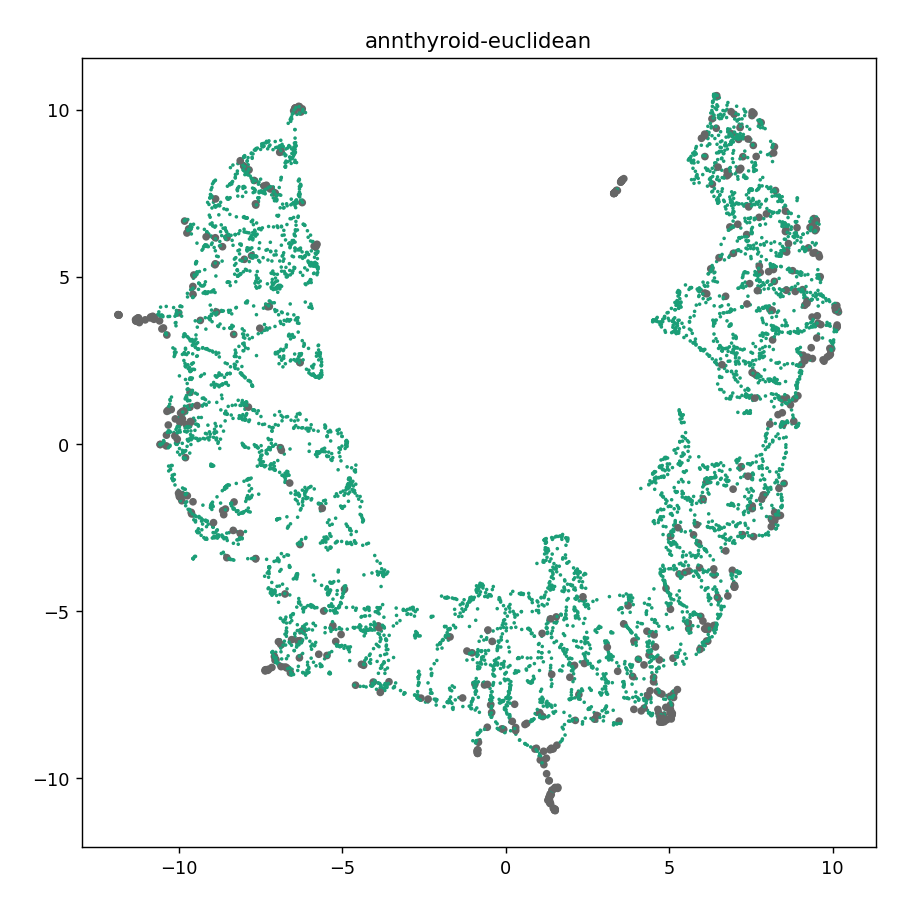
\includegraphics[width=2.5in]{images/umaps/annthyroid-euclidean-umap2d.png}
    \caption{UMAP embedding of Annthyroid data with the Euclidean distance function.}
    \label{fig:discussion:umap-annthyroid-euclidean}
\end{figure}

\subsubsection{APOGEE-2}
\label{subsec:methods:datasets:apogee-2}

euclidean, cosine, wasserstein-1d

\dots

\subsubsection{MaNGA}
\label{subsec:methods:datasets:manga}

euclidean, wasserstein-2d

\dots

\subsubsection{Silva 18S and variants}
\label{subsec:methods:datasets:silva-18s}

hamming, levenshtein

\dots

\subsubsection{ANN-Benchmarks suite}
\label{subsec:methods:datasets:ann-benchmarks-suite}

deep1b: cosine

fashion-mnist: euclidean

gist: euclidean

glove: cosine

kosarak: jaccard

mnist: euclidean

nytimes: cosine

sift: euclidean

last.fm: cosine

\dots

\subsection{Hardware}
\label{subsec:methods:hardware}

Specs of Ark, and maybe M1 MacBook Air and Dell XPS.


